\chapter{Framework \& Methodology}
\label{chap:methodology}

\section{Decentralized Framework Architecture}

The proposed decentralized multi-agent path planning framework is designed to enable each robot to make autonomous decisions based on local observations and communication with nearby agents. The overall architecture, illustrated in Figure~\ref{fig:framework_architecture}, comprises three main components: a Convolutional Neural Network (CNN) for local feature extraction from sensor data, an advanced Graph Neural Network (GNN) module based on Adaptive Diffusion Convolution (ADC) for inter-agent information aggregation and coordination, and a Multi-Layer Perceptron (MLP) that serves as an action policy network.

\begin{figure}[h]
    \centering
    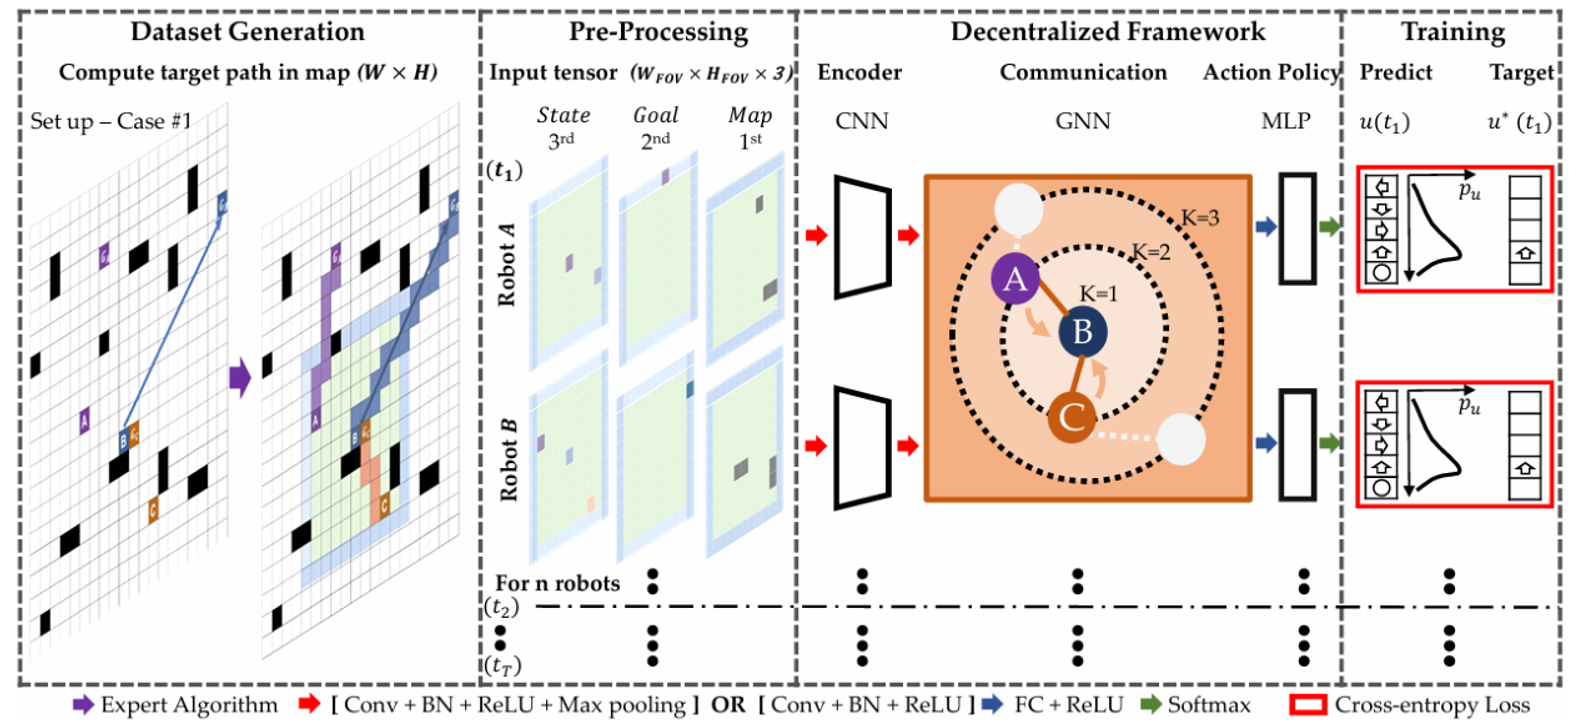
\includegraphics[width=1\textwidth]{images/framework_figure.png} % Replace with your actual figure file and name
    \caption{General Decentralized Framework Architecture for Multi-Agent Path Planning, highlighting the flow from observation to action through CNN, GNN, and MLP components.}
    \label{fig:framework_architecture}
    \cite{Li2021GNNCoordination}
\end{figure}

The core innovation of this thesis lies in the GNN component, where a standard fixed-hop GNN is replaced by an Adaptive Diffusion Convolution (ADC) mechanism. This enhancement allows for more flexible and adaptive communication strategies among robots. Figure~\ref{fig:adc_enhanced_architecture_detail} provides a more detailed view of this ADC-enhanced framework, emphasizing the components of the adaptive communication module.
\begin{figure}
    \centering
    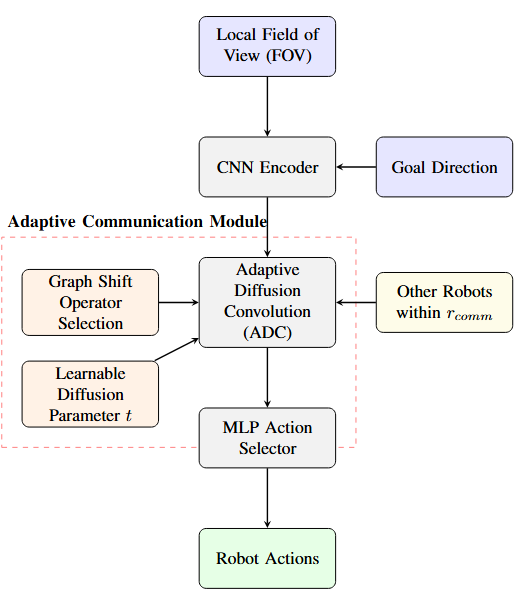
\includegraphics[width=0.7\textwidth]{images/block_diagram.png} % Replace with your actual figure file and name
    \caption{Detailed architecture of the ADC-enhanced MRPP framework.}
\label{fig:adc_enhanced_architecture_detail}
\end{figure}
\begin{comment}
\begin{figure}[t]
\centering
\begin{tikzpicture}[
    node distance=1.2cm,
    box/.style={rectangle, draw, minimum width=2.5cm, minimum height=1.2cm, text centered, rounded corners, text width=2.5cm},
    arrow/.style={thick,->,>=stealth},
    process/.style={rectangle, draw, fill=gray!10, minimum width=2.5cm, minimum height=1.2cm, text centered, rounded corners, text width=2.5cm},
    decision/.style={diamond, draw, fill=gray!10, minimum width=2.5cm, minimum height=1.2cm, text centered, text width=1.6cm}
]
% Nodes
\node[box, fill=blue!10] (fov) {Local Field of View (FOV)};
\node[process, below=of fov] (cnn) {CNN Encoder};
\node[process, below=of cnn] (gnn) {Adaptive Diffusion Convolution (ADC)};
\node[process, below=of gnn] (mlp) {MLP Action Selector};
\node[box, below=of mlp, fill=green!10] (action) {Robot Actions};
% Left side elements - Adjusted positioning to be closer
\node[box, left=0.8cm of gnn, fill=orange!10] (gsol) {Graph Shift Operator Selection};
\node[box, below=0.5cm of gsol, fill=orange!10] (diffusion) {Learnable Diffusion Parameter $t$};
% Right side elements - Adjusted positioning to be closer
\node[box, right=0.8cm of gnn, fill=yellow!10] (robots) {Other Robots within $r_{comm}$};
\node[box, right=0.8cm of cnn, fill=blue!10] (goal) {Goal Direction};
% Arrows
\draw[arrow] (fov) -- (cnn);
\draw[arrow] (goal) -- (cnn);
\draw[arrow] (cnn) -- (gnn);
\draw[arrow] (gnn) -- (mlp);
\draw[arrow] (mlp) -- (action);
\draw[arrow] (gsol) -- (gnn);
\draw[arrow] (diffusion) -- (gnn);
\draw[arrow] (robots) -- (gnn);
% Add a background container for the ADC part - Adjusted fit with label inside
\begin{scope}[on background layer]
\node[fit=(gsol) (diffusion) (gnn), draw=red!50, dashed, inner sep=0.4cm] (adc_box) {};
\end{scope}
% Place the label manually above the dashed box and to the left to avoid the arrow
\node[text=black, font=\bfseries, anchor=south west] at (adc_box.north west) {\textbf{Adaptive Communication Module}};
\end{tikzpicture}
\caption{Detailed architecture of the ADC-enhanced MRPP framework.}
\label{fig:adc_enhanced_architecture_detail}
\end{figure}
\end{comment}
\subsection{Observation Processing with Convolutional Neural Network}

Each robot is equipped with sensors that provide a local observation of its surroundings.The input is represented as a $W_{FOV} \times H_{FOV} \times 3$ tensor. This tensor, encompassing the local map, goal information (relative direction or position), and positions of other agents within the FOV, is processed by a CNN. The CNN acts as a feature extractor, designed to learn salient spatial features from this local observation, encoding information about obstacles, goal direction, and nearby agents into a compact feature vector.

The CNN architecture consists of a series of convolutional layers, batch normalization layers, ReLU activation functions, and max-pooling layers.
\begin{comment}
\begin{itemize}
    \item \textbf{Convolutional Layer 1:} \textit{X} filters of size \textit{Y}x\textit{Y} with stride 1 and padding 1, followed by Batch Normalization and ReLU activation.
    \item \textbf{Max-Pooling Layer 1:} Size \textit{Z}x\textit{Z} with stride \textit{S}.
    \item \textbf{Convolutional Layer 2:} \textit{... and so on for each layer}.
    \item \textbf{Flattening and Fully Connected Layer:} The output from the convolutional/pooling layers is flattened and passed through a fully connected layer to produce a feature vector $\mathbf{x}_i \in \mathbb{R}^F$ for each robot $i$.
\end{itemize}

This feature vector $\mathbf{x}_i$ summarizes the key information from robot $i$'s local perception and serves as its initial state representation for the communication module.
\end{comment}   
\subsection{Information Aggregation with Adaptive Diffusion Convolution (ADC)}
\label{subsec:adc_aggregation}

The GNN component is pivotal for enabling decentralized coordination by facilitating communication and information sharing among neighboring robots. In this work, we enhance the standard GNN approach by employing \textbf{Adaptive Diffusion Convolution (ADC)}, as detailed theoretically in Chapter~\ref{chap:background} . This replaces the fixed K-hop message passing scheme of conventional GNNs with a more flexible and learnable diffusion process.

The multi-robot system at any time step $t$ is modeled as a dynamic graph $G_t = (V, E_t)$. Here, $V$ is the set of $N$ robots, and an edge $(i, j) \in E_t$ exists if robot $j$ is within a predefined communication radius $r_{comm}$ of robot $i$. From this graph, a \textbf{Graph Shift Operator (GSO)} $\mathbf{T}_t$ is constructed, typically the symmetrically normalized adjacency matrix $\tilde{A}_t$ (as discussed in Section~\ref{sec:gsos}), which defines the local neighborhood structure for information propagation.

As illustrated in Figure~\ref{fig:adc_enhanced_architecture_detail}, the ADC module takes several inputs for each robot $i$:
\begin{itemize}
    \item The feature vector $\mathbf{x}_i$ (denoted as $H^{(l)}$ in the general layer formulation if $l=0$ or features from a previous ADC layer) extracted by its CNN.
    \item The GSO $\mathbf{T}_t$ representing the current communication graph.
    \item A \textbf{learnable diffusion time parameter $t$}, which is optimized during training. This parameter controls the extent of information propagation across the graph.
    \item Feature vectors from other robots within its communication range, which are implicitly used via the GSO.
\end{itemize}

The ADC layer then updates the robot's feature representation by propagating and aggregating information according to the graph heat kernel, approximated by a truncated Taylor series (Equation~\ref{eq:adc_approx_original} from Chapter~\ref{chap:background}):
\begin{equation}
H^{(l+1)} = \sigma \left( \left( \sum_{k=0}^{K_{trunc}} \theta_k(t) \mathbf{T}_t^k \right) H^{(l)} W^{(l)} \right)
\end{equation}
where $H^{(l)}$ is the input feature matrix (e.g., $X_t = [\mathbf{x}_1, \dots, \mathbf{x}_N]^T$ for the first ADC layer), $\theta_k(t) = e^{-t} \frac{t^k}{k!}$ are the learnable diffusion coefficients dependent on $t$, $K_{trunc}$ is the truncation order, $W^{(l)}$ is a learnable weight matrix for feature transformation, and $\sigma$ is a non-linear activation function (e.g., ReLU).

By learning the optimal diffusion time $t$, the ADC layer can dynamically adjust the "radius" of its receptive field on the graph, deciding how much information to aggregate from 1-hop, 2-hop, and further neighbors, weighted appropriately by the diffusion process. This adaptability is a key advantage over fixed-K GNNs, where the neighborhood size is predefined and static. The theoretical benefits of ADC, including stability and adaptive spectral filtering, are discussed in Section~\ref{sec:principal_results}.

The output of the ADC layer is a matrix $H_t' \in \mathbb{R}^{N \times G}$ (or $H^{(l+1)}$), where each row $\mathbf{h}'_i \in \mathbb{R}^G$ is the new, context-aware feature vector for robot $i$. This vector $\mathbf{h}'_i$ incorporates information not only from its local CNN-processed observation but also from relevant teammates, scaled by the learned diffusion process.

\subsection{Action Policy Generation with Multi-Layer Perceptron (MLP)}

The final component in the robot's decision-making pipeline is an MLP, which functions as the action policy network. It takes the aggregated and context-aware feature vector $\mathbf{h}'_i$ (output from the ADC module) for robot $i$ as input. The MLP then outputs a probability distribution over a predefined discrete set of actions. For this MRPP task, we typically consider five actions: \{'move forward/up', 'move backward/down', 'move left', 'move right', 'stay idle'\}.

The MLP is designed to map the rich feature representation $\mathbf{h}'_i$ to an optimal action choice that helps the robot navigate towards its goal while avoiding collisions. The MLP architecture usually consists of one or more hidden layers with non-linear activation functions (e.g., ReLU), followed by an output layer with a Softmax activation function. The Softmax function ensures that the output is a valid probability distribution across the available actions.


\begin{itemize}
    \item \textbf{Linear Layer 1:} Input size $G$ (from ADC output), Output size \textit{M}, followed by ReLU activation.
    \item \textbf{Linear Layer 2 (Output Layer):} Input size \textit{M}, Output size 5 (number of actions), followed by Softmax activation.
\end{itemize}

The action $\mathbf{u}_i$ for robot $i$ at time step $t$ is then selected by sampling from this output probability distribution, or by choosing the action with the highest probability (argmax) during deterministic execution.

\section{Imitation Learning Methodology}

The proposed ADC-enhanced framework is trained using imitation learning. Specifically, we employ supervised learning where the model learns to mimic expert demonstrations. The expert, in this case, is the Conflict-Based Search (CBS) algorithm, which is capable of generating optimal or near-optimal path plans for multi-robot systems.

\subsection{Training Dataset and Loss Function}

The training dataset $\mathcal{D} = \{(\mathcal{Z}^{(j)}, \mathcal{U}^{*(j)})\}_{j=1}^{M_{scen}}$ consists of $M_{scen}$ scenarios. Each scenario $j$ provides a sequence of expert actions $\mathcal{U}^{*(j)} = \{U_1^{*(j)}, U_2^{*(j)}, \dots, U_{TMP^{*(j)}}^{*(j)}\}$ and the corresponding sequence of local observations $\mathcal{Z}^{(j)} = \{Z_1^{(j)}, Z_2^{(j)}, \dots, Z_{TMP^{*(j)}}^{(j)}\}$ for all $N$ robots over the makespan $TMP^{*(j)}$ of the expert solution. These datasets are generated as detailed in Chapter~\ref{chap:dataset}.

The model, parameterized by $\Theta$ (which includes weights of the CNN, ADC layer including the learnable $t$, and MLP), is trained to minimize the cross-entropy loss between its predicted action probability distribution $\pi_{\Theta}(\mathbf{z}_{i,t}, G_t)$ and the expert's chosen action $\mathbf{u}^*_{i,t}$ for each robot $i$ at each time step $t$. The total loss function over the dataset is:
\begin{equation}
\mathcal{L}(\Theta) = \sum_{j=1}^{M_{scen}} \sum_{t=1}^{TMP^{*(j)}} \sum_{i=1}^{N} L_{CE}(\mathbf{u}^*_{i,t}, \pi_{\Theta}(\mathbf{z}_{i,t}^{(j)}, G_t^{(j)}))
\end{equation}
where $\mathbf{z}_{i,t}^{(j)}$ is the local observation for robot $i$ at time $t$ in scenario $j$, $G_t^{(j)}$ is the communication graph at that time, and $L_{CE}$ denotes the standard cross-entropy loss.

\subsection{Training Procedure}

The training procedure involves the following iterative steps:

\begin{enumerate}
    \item \textbf{Initialization:} Initialize the parameters $\Theta$ of the CNN, ADC (including $t$), and MLP networks, typically with random values or pre-trained weights if applicable.
    \item \textbf{Batch Processing:} For each training epoch, iterate through the training dataset in batches.
    \item \textbf{Forward Pass:} For each scenario (or segment of a trajectory) in a batch, and for each time step $t$:
        \begin{enumerate}
            \item Each robot $i$ processes its local observation $\mathbf{z}_{i,t}$ using the CNN to obtain feature vector $\mathbf{x}_{i,t}$.
            \item Construct the communication graph $G_t$ and its corresponding GSO $\mathbf{T}_t$ based on current robot positions and $r_{comm}$.
            \item Aggregate information using the ADC layer (with the current learned $t$) to obtain context-aware feature vectors $\mathbf{h}'_{i,t}$.
            \item Generate action probability distributions $\pi_{\Theta}(\mathbf{z}_{i,t}, G_t)$ using the MLP for each robot.
        \end{enumerate}
    \item \textbf{Loss Calculation:} Calculate the cross-entropy loss $\mathcal{L}_{batch}(\Theta)$ for the current batch using the predicted action distributions and the expert actions.
    \item \textbf{Backpropagation and Optimization:} Compute the gradients of $\mathcal{L}_{batch}(\Theta)$ with respect to all learnable parameters $\Theta$ (including the diffusion time $t$ in ADC) using backpropagation. Update the parameters using an optimization algorithm, such as Adam \cite{Kingma2014Adam}, to minimize the loss.
    \item \textbf{Iteration and Convergence:} Repeat steps 2-5 for a predefined number of epochs or until the loss on a separate validation set converges or shows no significant improvement (early stopping).
\end{enumerate}

\subsection{Dataset Aggregation with Online Expert (DAgger)}

To further enhance the robustness of the learned policy and mitigate issues arising from covariate shift (where the distribution of states encountered by the learned policy during execution differs from the expert's state distribution), a dataset aggregation technique like DAgger (Dataset Aggregation) \cite{Ross_et_al_2011} can be optionally employed.

The DAgger procedure involves:
\begin{enumerate}
    \item Train an initial policy $\pi_0$ on the expert dataset $\mathcal{D}_0$.
    \item For $k=0, 1, \dots, K_{DAgger}-1$:
        \begin{enumerate}
            \item Execute the current policy $\pi_k$ in the environment to collect a set of trajectories and observations.
            \item For the states encountered by $\pi_k$, query the expert planner (CBS) to obtain the optimal actions.
            \item Aggregate these new (state, expert\_action) pairs into the dataset: $\mathcal{D}_{k+1} = \mathcal{D}_k \cup \{\text{new expert-labeled data}\}$.
            \item Train a new policy $\pi_{k+1}$ on the aggregated dataset $\mathcal{D}_{k+1}$.
        \end{enumerate}
    \item The final policy is one of the $\pi_k$ (e.g., $\pi_{K_{DAgger}}$) or a mixture.
\end{enumerate}
This iterative process allows the policy to learn from its own mistakes by querying the expert in regions of the state space it explores, leading to a more robust policy that performs well even when it deviates from the expert's original trajectories.

\section{Decentralized Online Execution and Collision Shielding}

Once the ADC-enhanced framework is trained, it is deployed for decentralized online path planning. During execution, each robot independently and concurrently performs the following steps at each discrete time step:

\begin{enumerate}
    \item \textbf{Local Observation:} Robot $i$ obtains its local observation map $Z_{i,t}$ from its sensors.
    \item \textbf{Feature Extraction:} Process $Z_{i,t}$ through its CNN to extract the feature vector $\mathbf{x}_{i,t}$.
    \item \textbf{Communication and Aggregation:}
        \begin{itemize}
            \item Identify neighboring robots within communication range $r_{comm}$.
            \item Construct (or update) its local view of the communication graph $G_t$ and the GSO $\mathbf{T}_t$.
            \item Exchange necessary information (e.g., feature vectors $\mathbf{x}_{j,t}$ or intermediate representations if using multi-layer ADC) with direct neighbors.
            \item Perform information aggregation using its ADC layer with the learned diffusion time $t$ (which is now a fixed parameter of the trained model) to obtain the context-aware feature vector $\mathbf{h}'_{i,t}$.
        \end{itemize}
    \item \textbf{Action Selection:} Generate action probabilities using its MLP based on $\mathbf{h}'_{i,t}$ and select an action $\mathbf{u}_{i,t}$ (e.g., by taking the argmax or sampling from the distribution $\pi_{\Theta}$).
    \item \textbf{Collision Shielding (Safety Mechanism):} Before executing the chosen action $\mathbf{u}_{i,t}$, apply a collision shielding mechanism. This mechanism checks if the intended action would lead to an immediate collision with static obstacles or with other robots (based on their predicted or recently communicated planned actions). If a collision is predicted, the action $\mathbf{u}_{i,t}$ is overridden, typically with an 'idle' or 'stay' action, to ensure safety.
    \item \textbf{Execution and State Update:} Execute the final (potentially shielded) action. This updates the robot's position in the environment. The robot then proceeds to the next time step, repeating the cycle.
\end{enumerate}

This fully decentralized execution process allows each robot to navigate autonomously, making decisions based purely on its local perceptions and limited communication with nearby peers. The collision shielding layer acts as a crucial safety guarantee, augmenting the learned policy to prevent basic types of collisions.

\section{Chapter Summary}

This chapter has presented the framework and methodology for decentralized multi-agent path planning using an Adaptive Diffusion Convolution (ADC) enhanced Graph Neural Network. We detailed the overall architecture, including the CNN for local perception, the novel ADC module for adaptive inter-agent communication, and the MLP for action selection. The imitation learning approach, leveraging expert demonstrations from Conflict-Based Search (CBS) for training, was described, along with an optional DAgger-like procedure for further policy refinement. Finally, the decentralized online execution protocol, incorporating a vital collision shielding mechanism for safety, was outlined. This comprehensive framework aims to achieve efficient, scalable, and safe navigation for multi-robot systems in complex environments by enabling robots to learn adaptive communication strategies. The subsequent chapters will discuss the dataset generation process, experimental setup, and the empirical results obtained with this framework.